% !TeX root = ../main.tex
% %%%%%%%%%%%%%%%%%%%%%%%%%%%%%%%%%%%%%%%%%%%%%%%%%%%%%%%%%%%%%%%%%%%%%%%%%%%%%%
% Introduction
\chapter{Introduction}
\label{chap:introduction}

Tendo a robótica um grande impacto no mundo em que vivemos, a qualidade do software utilizado por 
robôs é algo a que deveríamos dar bastante importância. As especificações deste tipo de software e 
como são feitos testes para verificar a sua qualidade diferenciam-se bastante da norma. Testes 
automáticos são pouco utilizados na área devido a diversos factores, tendo em conta estes factores 
pretende-se criar uma ferramenta que promova uma fácil e confiável utilização de testes automáticos 
na área, esta dependerá de uma linguagem descritiva de alto nível que captura certas propriedades de 
um robô em conjunto com uma ferramenta de criação de cenários de teste.
\alcides{Deves separar em parágrafos ideias diferentes. A última frase também está muito comprida, e devia ser separada em duas.}

% ------------------------------------------------------------------------------
% Motivation
\section{Motivation}
\label{sec:motivation}
Atualmente robôs são vastamente utilizados industrialmente (medicina, agricultura, etc.) ou como 
forma de lazer (competições, uso pessoal, etc.), a tendência é para a sua utilização continuar a 
aumentar à escala mundial. 

\alcides{utilizados não só industrialmente, mas também como em forma de lazer. (ponto final. é uma ideias diferente) A tendência é para a sua...}

As tarefas a serem realizadas por robôs tendem a ser repetitivas e/ou 
bastante específicas, também o seu software tende a ser diferente do software convencional, no 
sentido em que o seu sistema Ciber-Físico é não-determinístico e não-confiável, algumas razões são o 
facto de robôs interagirem diretamente com o seu ambiente e os seus sensores poderem devolver valores 
imprecisos, isto porque o próprio ambiente pode ser difícil de prever. Como resultado a noção de que 
uma tarefa ou movimento esteja correcto é difícil de conceber para um robô. 

\alcides{Temos de começar novo parágrafo aqui. Já justificamos o porquê do problema ser dificil.}


\alcides{Falas em testes automáticos, mas deverias primeiro identificar soluções para evitar isto. Introduzir primeiro testes, depois testes automáticos.}

Consequentemente testes 
automáticos são difíceis de realizar nesta área, de facto atualmente a grande maioria dos testes 
realizados em robôs necessitam de supervisionamento humano seja o teste feito no mundo real ou numa 
simulação, identifica-se assim que existe um espaço para melhoramento na área de testes para robôs 
através de testes automáticos optimizados com o objectivo de melhorar a qualidade destes sistemas.

\section{Problem Statement}
\label{sec:problem}

\alcides{Metade do parágrafo está na primeira frase. Que é enorme! Deverias reestruturar em frases mais pequenas, com ideias directas.}

Existem vários desafios ao fazer testes em robôs, entre custos, complexidade, integração de hardware, 
existindo diferentes escolhas a fazer quando se vai testar um robô, estas escolhas têm tradeoffs, 
enquanto que testes usando simulações são uma abordagem promissora para a automação na área de testes 
em robótica existe desconfiança na precisão e validade dos resultados, de maneira que, apesar de 
perigoso e por vezes possivelmente caros, testes em robôs no mundo real continuam a ser escolhidos. 
Sejam os testes feitos em simulação ou no mundo real a maioria deles são feitos recorrendo a 
supervisionamento humano, isto porque identificar se o robô realiza o comportamento correcto ou 
esperado pode ser algo de difícil para um robô de compreender. Verifica-se então que testes automáticos 
na área da robótica para além de serem atualmente pouco confiáveis são também difíceis de implementar, 
resultando assim num problema na qualidade do software.~\cite{TestRob} \todo {O ponto vem depois da citação.}

% ------------------------------------------------------------------------------
% Objectives
\section{Objectives}
\label{sec:objectives}

\alcides{A primeira frase tem de ser reescrita. Não facilitas developers, mas facilitas a criação de testes automáticos.}
Este trabalho tem como objectivo dar a mostrar o potencial de testes automáticos em robótica e facilitar 
developers do ramo na realização de testes nos seus robôs. Para atingir este objectivo propõe-se criar 
um mecanismo de monitorização de certos componentes do robô durante e/ou após a execução de um teste. 


\alcides{Queres arbitrários em vez de aleatórios. Acho que devias começar com o desenho de uma linguagem de alto nível para especificação de propriedades de sistemas robóticos. Depois um compilador que traduzia essa linguagem num mecanismo de monitorização. Mas a linguagem devia ser o ponto inicial. Acho que falar do GZScenic ainda não é relevante aqui.}
Estes componentes do robô não serão aleatórios mas sim definidos com a ajuda de uma nova linguagem de 
alto nível, o objectivo é conseguir-se descrever as propriedades do robô com ajuda desta linguagem, 
deste modo se o robô não seguir as propriedades definidas durante um teste o seu comportamento não será 
correcto. Será também preciso criar cenários de teste específicos e aleatórios para o robô de uma forma 
automática, já existindo uma linguagem para este efeito (GzScenic)~\cite{GzScenic} pode-se tirar partido 
da mesma.
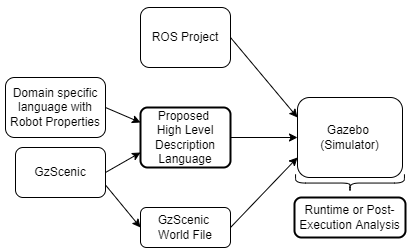
\includegraphics{images/intro_diag.png}
\alcides{A imagem devia estar como uma figura. A parte do GzScenic ainda não é relevante. Falta uma legenda dos vários tipos de componentes da imagem.}
\alcides{Neste ponto ainda não apresentaste o ROS. Acho relevante dar uma pequena introdução ao que é, para se perceber aqui o esquema.}

\section{Contributions}
\label{sec:contributions}

The expected contributions of this thesis are below enumerated.

Alterar a prespectiva da utilização de testes automáticos na área da robótica.

Criar uma ferramenta simples de usar que permite realizar testes automáticos na área da robótica.


\alcides{Aqui pretendem-se coisas mais concretas: 1. Definição de uma linguagem de alto nível para especificação de propriedades de robots. Depois um compilador dessa linguagem para monitorização. Depois uma avaliação da capacidade desta solução modelar vários problemas relevantes na robótica.}

% ------------------------------------------------------------------------------
% Structure of the document
\section{Structure of the document}
\label{sec:structure}

The document is organized as follows:

\begin{itemize}
    \item Section 1...
    \item Section 2...
    \item Section 3...
\end{itemize}

